\chapter{Introduction}

- deepfake is buzzword (no agreed-upon technical definition)
- still growing thread for sociaty
- huge research over past years
- reason for creating this framework

\chapter{Deepfakes}

The creation of fake media and their detection have been a problem since photography was invented. Digital photography or video with tools such as GIMP, Adobe Photoshop or Adobe After Effects allows more people to create fakes than before, still some experience in this area is needed. Media that have been modified or otherwise manipulated are called synthetic media, and they do not depend on whether it is an analogue or digital medium. Deepfakes also fall under this category \cite{IncreasingThreatofDeepfakeIdentites}. Tools powered by deep learning allow unexperienced users to easily create trusted fakes. 

The quality of deepfakes reached a level when a trained person or even an experienced researcher in this field has a problem of spotting them. This fast development allows creating realistically looking assets to art photography or movie production, unfortunately, it can be used for malicious purposes like creating fake porn videos to blackmail people or manipulate public via fake news. There are many use cases where deepfakes can be applied.

It is putting huge pressure on researchers to develop new forensics tools or any technology which will prevent malicious usage of deepfakes. As mentioned before, creating fakes is not new, and a whole field of study engaged in spotting fakes and developing techniques over 15 years. Despite continuous research efforts in the past, the advent of deep learning changed the rules of the game. \cite{MediaForensicsandDeepFakes}

\section{Human capabilities of deepfake detection}

The human ability to recognize fake materials from the originals is in contradiction to their quality. Korshunov and Marcel confirmed this in their research. They created a questionnaire containing several videos, and the subject (interviewee) had to answer after watching the video whether the person in the video was genuine, fake, or they are uncertain. The videos were manually divided into five categories (very easy, easy, moderate, difficult, and very difficult, original). 

Videos were split into several categories manually by researchers probably without usage of any metrics but based on their experience and feelings. Afterwards ANOVA test shows there is an overlap in several categories, so several videos could be moved to different category. However, the categories are still significantly different. 

The results of test in Fig. \ref{fig:subjective_answers} certainly demonstrate that people's recognition ability decreases significantly as the quality of deepfakes increases. Also, the audience of this test knows they are looking for fakes, otherwise we can expect worse results if there will be unsuspected audience (e.g. deepfakes on social media). It is quite alarming that the correct answers in the category of “very easy” reach only 71,1 \%. The quality of deepfake increases over time, thus it can be expected that human recognition ability will continue to decrease. \cite{TheThreatOfDeepfakes}

\begin{figure}[H]
    \begin{subfigure}[h]{.475\linewidth}
        \centering
        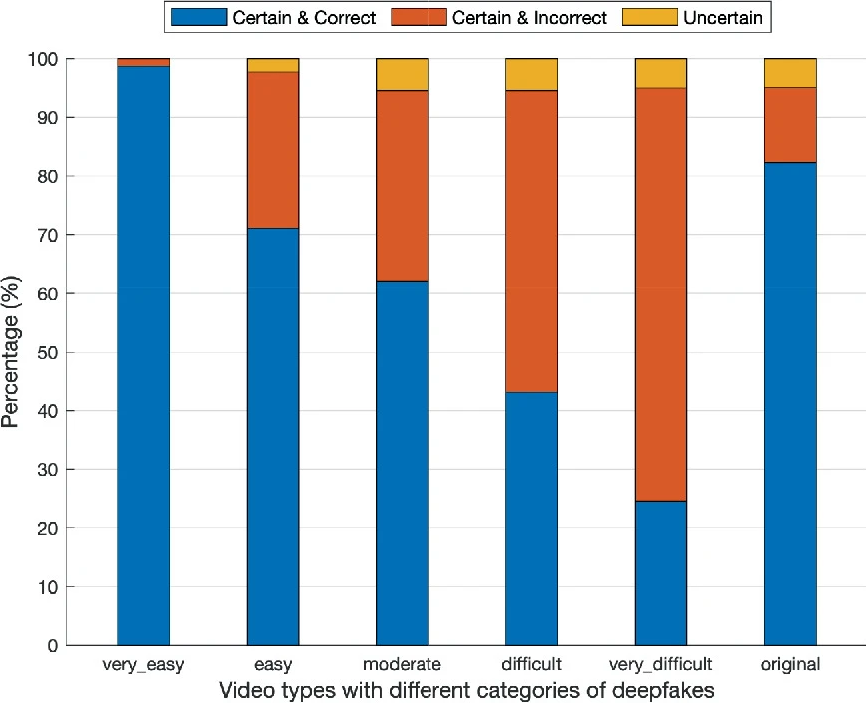
\includegraphics[width=1\linewidth]{other-fig/subjective_answers_a.png}
        \caption{Subjective answers}
    \end{subfigure}
    \hfill
    \begin{subfigure}[h]{.475\linewidth}
        \centering
        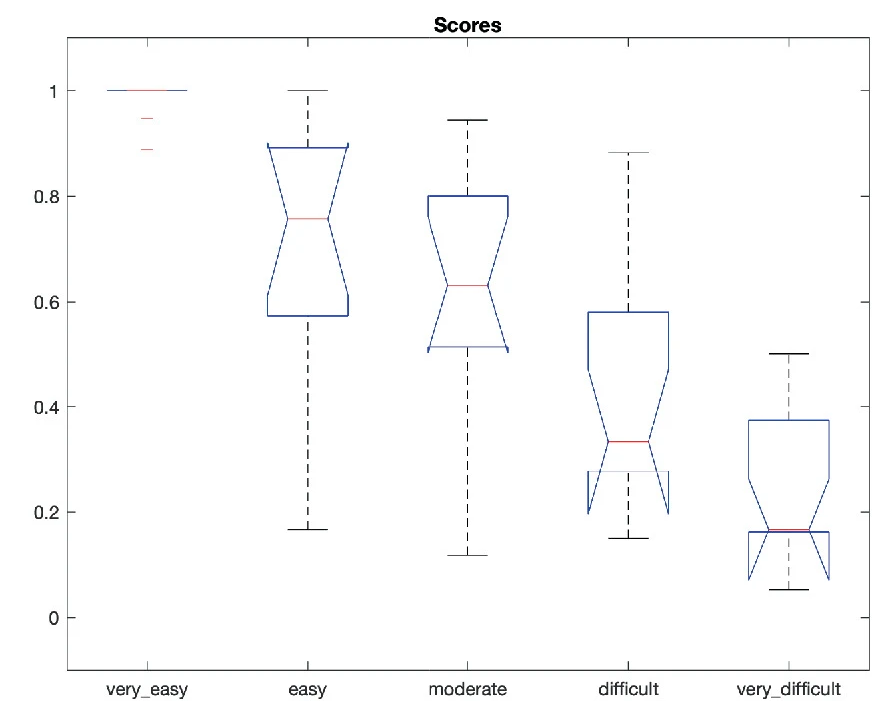
\includegraphics[width=1\linewidth]{other-fig/subjective_answers_b.png}
        \caption{ANOVA test}
    \end{subfigure}
    \caption{Subjective answers and median values with error bars from ANOVA test for different deepfakehttps://www.overleaf.com/project/6373f30660c2425f4720defb categories. Retrieved from \cite{TheThreatOfDeepfakes}.}
    \label{fig:subjective_answers}
\end{figure}

Another research tested only recognition of audio tracks and they were comparing humans versus computer programmes. Attendees had a correct classification between fakes and origins 67 \% after the first several rounds. Their accuracy increased while listening and answering to more tracks, but the value stabilizes to 80 \%. On average, trained AI performs about 10 \% better than human, but this result highly depends on difference of learning and test dataset. Still, it shows that the computer can outperform humans in spotting deepfakes. \cite{HumanPerceptionAudio}

\section{Potentional risks}

Humans are not good at recognizing deepfakes, but “why should we be worried?”. Almost every technology humankind created could be used for good or bad – deepfake is no exception. There are plenty different deepfake categories, and each has its own attack vector or use case. This section is describing potential risks of those categories and their closer description will be covered in next section \ref{section:deepfakes_creation}.

Deepfakes are about gaining someone’s trust or influence him. For the last couple of years there has been an increasing trend of scamming people, mostly via phone or computer \cite{HybridVishingAttacksSkyrocketing}. Targeting only one person/victim, for example, to gain their money or information. Those attacks are getting better and more credible and using deepfake to impersonate close friend of victim could be next step how to improve it, if it is not already happening.

Creating “fake news” to influence a large audience is the most common use case of deepfakes because we live in an information era. There are many targets of “fake news” such as rigging elections, demoralizing military units, or manipulating the stock market. In this case, politicians, celebrities, and significant personalities will be used in deepfakes to influence audience. We can only imagine what one person or high quality deepfake can change with enough media reach. For example, after one tweet from Elon Musk about Tesla’s stock, sends shares down more than 10 \% almost immediately \cite{ElonMusksTweets}. \cite{IncreasingThreatofDeepfakeIdentites}

A real example of deepfake is famous video with Barak Obama insulting Donald Trump, which should spread awareness regarding the fast developing category of new thread \footnote{\url{https://www.buzzfeed.com/craigsilverman/obama-jordan-peele-deepfake-video-debunk-buzzfeed}}. Several years later another video stating Volodimir Zelenskyj talking about surrendering, it was proved that it is a manipulated video, and its purpose was to demoralize Ukraine army and make them capitulate \footnote{\url{https://www.youtube.com/watch?v=X17yrEV5sl4}}.

Another field where deepfakes could be used is to tricky biometrics systems in which the attacker is a different person to the gain access (banking, building, ...) \cite{DawnOfTextDependentSociety}, to secured equipment, etc. It was proven that biometrics system is not ready to deal with deepfakes, and it will probably require to add a new module to authentication pipeline which will be detecting deepfakes \cite{DigitalFaceManipulation}. Face or voice biometrics recognition systems are in greatest danger. The falsification of documents is related to this topic and there was a case of smuggling people across borders with an official passport containing morphed photos of two individuals \cite{FaceMorphingAttackDetectionMethods}.

These cases are only the tip of the iceberg, and in the future, everyone should ask if video on social media with film celebrity is real or even worse, if the evidence in courts is trustworthy or not. The solution for this is using tools capable of detecting deepfakes. Those tools have to be created with caution for unskilled users.

\section{Types of deepfakes and their creation process}
\label{section:deepfakes_creation}

There are plenty of methods on how to create deepfakes, and as its name suggests some of them are based on deep neural networks, but not exclusively.  This section describes most common types of learning networks used for creating image/video or voice deepfakes. One of the most popular types for face deepfakes is Generative adversarial network (GAN), and it is used to create completely new faces or face manipulations.

Each method leaves traces in the medium that can then be detected. This is one way to recognize deepfakes so understanding process of creation is an advantage. Detecting will be described in more detail in Chapter \ref{chapter:deepfake_detectoin}.

\subsection{Neural networks}

All the facts regarding neural networks were retrieved from \cite{CreationandDetectionofDeepfakes}. Neural networks are composited from neurons arranged in layers, and each layer is connected sequentially via synapses. Synapses are weighed, and the process of finding the proper value of all weights is called a learning neural network. To obtain results from the input of \(n\)-dimensional \(x\) process \texttt{forward-propagation} is used to propagate \(x\) through each layer.

Input to layer is vector \(a\) of values calculated by previous layer or in case of first layer \(x\) itself. That means result of each layer is also vector calculated by activation function \(f(a*W+b)\), where \(f\) is activation function (Sigmod, ReLU, etc.), \(a\) is input vector, \(W\) is matrix of weights between layers \(i\) and \(i+1\) and b is dimensional bias. Dimensional bias is a constant offset that helps the network shift the activation function toward the positive or negative side \cite{NeuralNetworkBias}.

Now let’s consider the neural network \(M\) as a black box and denote its execution as \(M(x) = y\). Supervise learning to train \(M\) is using paired samples with from \((x_i, y_i)\) and loss function \(L\) is defined. Loss function is to generate a signal at the output of \(M\) and propagate him back to find error of each weight in synapses.

Optimalization algorithms such as gradient descent are then used to calculate new weights of \(M\) for the number of epochs. As a result of this process, the network learns the function \(M(x_i) \approx y_i\) and is capable of making prediction on unseen data. More detailed descriptions of this could be found in the work of Y. Mirsky and W. Lee \cite{CreationandDetectionofDeepfakes}.
\\\\
Next list shows types of neural networks used for generating deepfakes \cite{CreationandDetectionofDeepfakes}:

\begin{itemize}
\item Generative Adversarial Networks (GAN) – Consist of two neural networks working against each other. One layer is generator and second is discriminator. Generator producing fake features trying to fool discriminator, on the other hand, discriminator is learning to distinguish between real sample and fake one.
\item Encoder-Decoder networks (ED) – Contains at least two networks, encoder and decoder. It has narrowed layers towards its center. If encoder \(En\) and decoder \(De\) are symmetric and they are trained as \(De(En(x)) = x\), then the network is called autoencoder. Generating deepfakes using ED trained with function \(De(En(x)) = x_g\), where \(x_g\) is fake generated features. There is possibility to use multiple different ED chained after each other or using specific variant of ED called variational autoencoder.
\item Convolutional Neural Network (CNN) – CNN is learning pattern hierarchies in the data. For deepfakes purposes, it learns filters applied over the input and forming an abstract feature map as the output.
\item Recurrent Neural Networks (RNN) – RNN can handle variable length data and it is remembering stat after processing which can be used in next iteration. RNN are mostly used in audio.
\end{itemize}

Each architecture has its own subcategories that have small modifications or using some techniques from different architecture. All above mentioned neural networks types are shown in \ref{fig:nns_architecture} and \ref{fig:cnn_architecture} 

\begin{figure}[H]
    \centering
    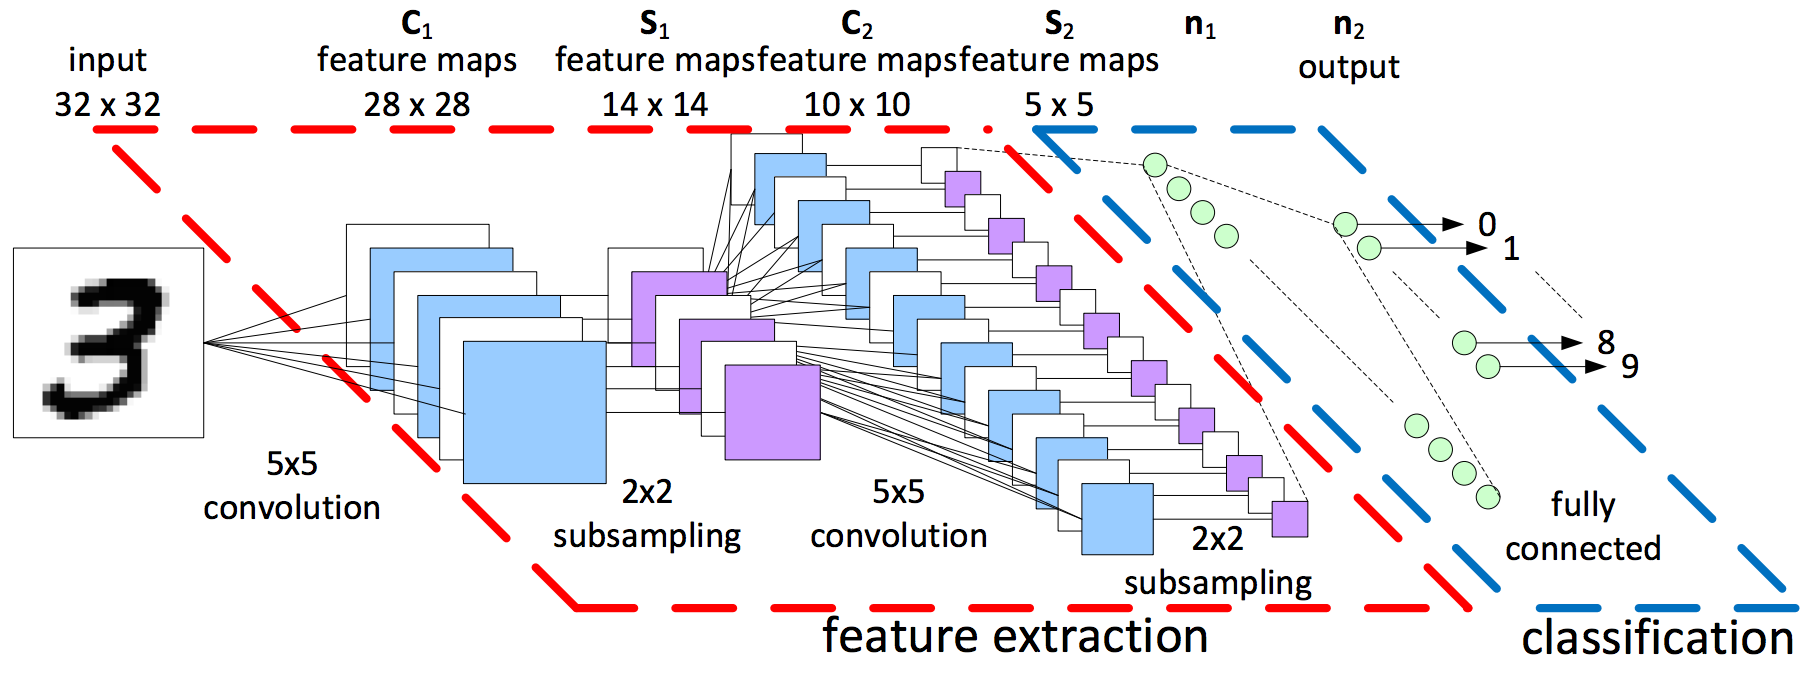
\includegraphics[width=.7\linewidth]{other-fig/cnn.png}        
    \caption{Architecture of convolutional neural network. Retrieved from \cite{CNNArchitecture}.}
    \label{fig:nns_architecture}
\end{figure}

\begin{figure}[H]
    \centering
    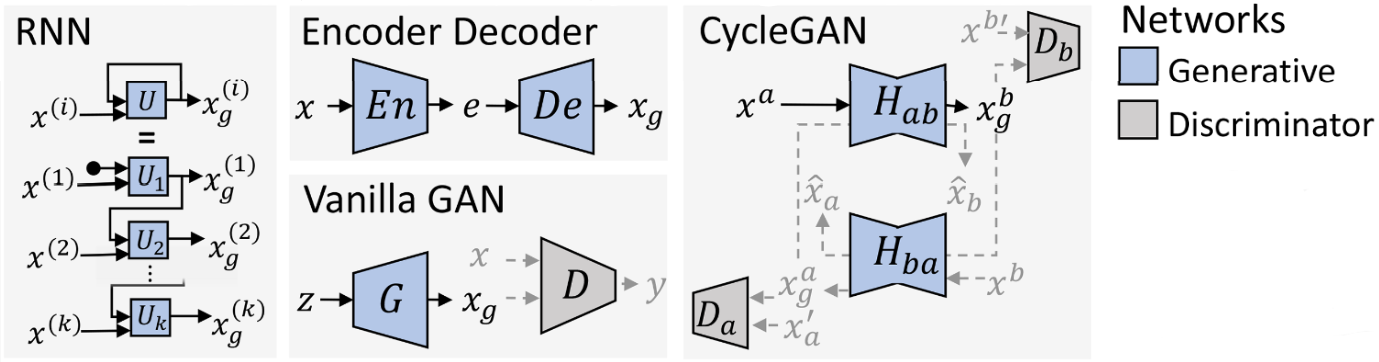
\includegraphics[width=.65\linewidth]{other-fig/nns.png}        
    \caption{Basic neural network architectures (RNN, ED, GAN). Retrieved from \cite{CreationandDetectionofDeepfakes}.}
\label{fig:cnn_architecture}
\end{figure}

\subsection{Voice deepfakes}

Speech synthesis is divided into two categories based on input data. Text to speech (TTS) converts written text to artificial speech and second category is called voice conversion (VC). The voice conversion consumes source voice, and both methods produce synthesis voice saying desired phrases specified by the input. \cite{ApplicabilityOfDeepfakes}

Voice deepfakes are used independently or with deepfake video (e.g. full puppet). Creating synthesis voice is computationally challenging and one of the goals is making real-time voice conversion. There are several projects that are trying to accomplish this \footnote{\url{https://github.com/SolomidHero/real-time-voice-conversion}} \footnote{\url{https://www.resemble.ai/speech-to-speech/}}.

\subsection{Image or video deepfakes}

The list of the following deepfakes is based on the work R. Tolosana, et al. \cite{IntroductionToDigitalFaceManipulation}:

\begin{itemize}
\item Identity swap – Replacing the face of subject with the face of target as shown in Fig. \ref{fig:idenity_swap}. There are two different approaches, classical computer graphics-based technique and deep learning technique. Generally, the process of swap could be described as face detection, cropping, extraction of intermediate representations, synthesis of new face, and blending the generated face.
\begin{figure}[H]
    \centering
    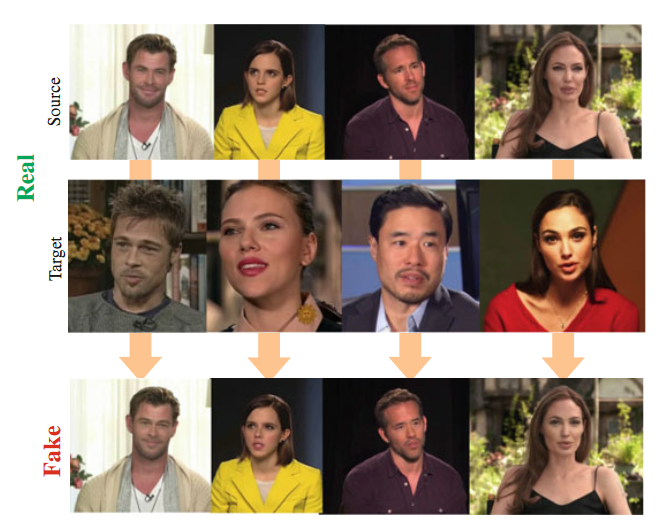
\includegraphics[width=.66\linewidth]{other-fig/idenity_swap.png}        
    \caption{Examples of real and fake identity swap images. Retrieved from \cite{IntroductionToDigitalFaceManipulation}.}
\label{fig:idenity_swap}
\end{figure}

\item Full puppet – Method related to identity swap allows creation of so-called puppet. One person (master) is source of facial expression and body movements that are mapped onto target person as shown in Fig. \ref{fig:full_puppet}. \cite{IncreasingThreatofDeepfakeIdentites}
\begin{figure}[H]
    \centering
    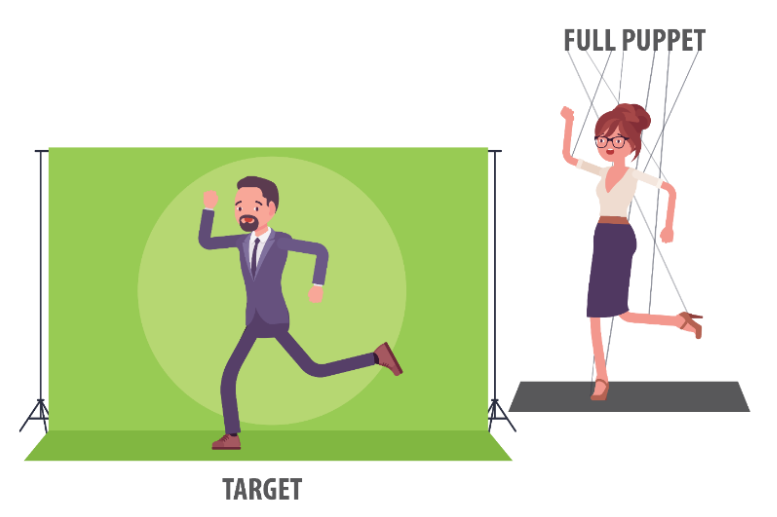
\includegraphics[width=.43\linewidth]{other-fig/full_puppet.png}        
    \caption{Full puppet technique visualisation. Retrieved from \cite{TheThreatOfDeepfakes}.}
\label{fig:full_puppet}
\end{figure}

\item Morphing – It is a type of manipulation that is used to create artificial biometric face samples. Final face contains resemble biometric information of two or more individuals. It should be possible to be successfully verified by biometrics systems for all individuals who were source for given deepfake. Fig. \ref{fig:morphing} shows an example of a morphed image.
\begin{figure}[H]
    \centering
    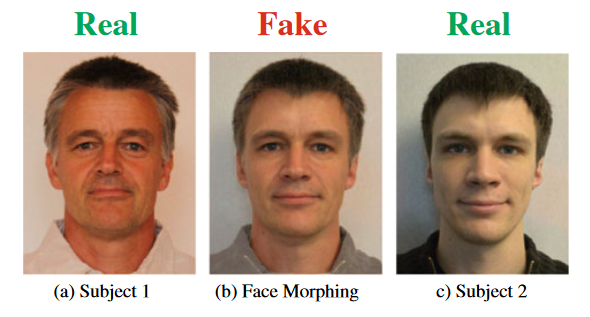
\includegraphics[width=.45\linewidth]{other-fig/morphing.png}        
    \caption{Examples of fake morphed identity from Subject 1 and Subject 2. Retrieved from \cite{IntroductionToDigitalFaceManipulation}.}
\label{fig:morphing}
\end{figure}

\item Attribute manipulation – Face editing or face retouching technique involves modifying some attributes such as length or color of hair, color of skin, sex, age, adding glasses or other artefacts, and more. Fig. \ref{fig:attribute_manipulation} shows an example of this technique.
\begin{figure}[H]
    \centering
    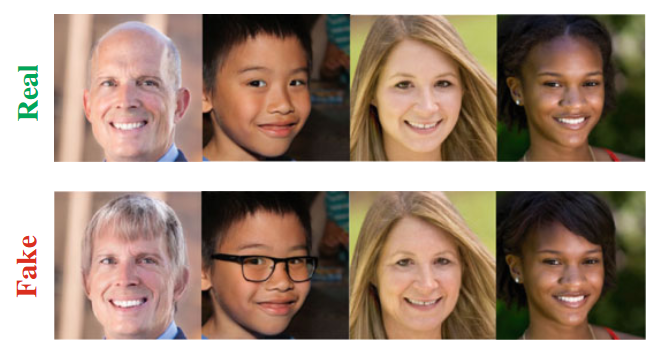
\includegraphics[width=.55\linewidth]{other-fig/attribute_manipulation.png}        
    \caption{Examples of real and fake attribute manipulation category. Retrieved from \cite{IntroductionToDigitalFaceManipulation}.}
\label{fig:attribute_manipulation}
\end{figure}

\item Expression swap – Modifying facial expression of the subject as shown in Fig. \ref{fig:expression_swap}. This technique is used as one of part for full puppet.
\begin{figure}[H]
    \centering
    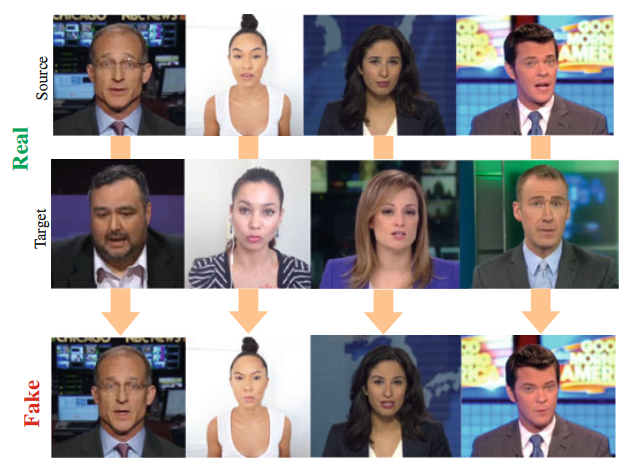
\includegraphics[width=.64\linewidth]{other-fig/expression_swap.png}        
    \caption{Examples of real and fake expression swap category. Retrieved from \cite{IntroductionToDigitalFaceManipulation}.}
\label{fig:expression_swap}
\end{figure}

\item Audio/text to video – This method related to expression swap synthesising facial expression from audio or text. It is also known as lip-sync deepfakes. Diagram in Fig. \ref{fig:audio_to_video} shows how this method works.
\begin{figure}[H]
    \centering
    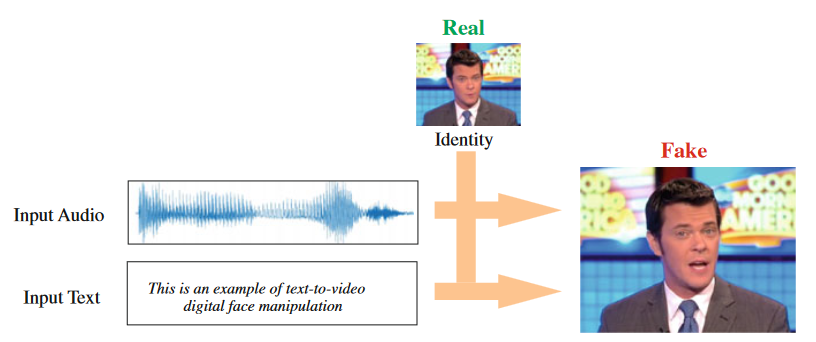
\includegraphics[width=.65\linewidth]{other-fig/audio_to_video.png}        
    \caption{Examples of real and fake audio/text to video fake category. Retrieved from \cite{IntroductionToDigitalFaceManipulation}.}
\label{fig:audio_to_video}
\end{figure}
\end{itemize}

Creating deepfakes nowadays is complex task and many deepfakes is using more techniques so that they could be included into more than one category. Attackers could create deepfake that will fall under identity swap category and after that use attribute manipulation to tune final results.

\chapter{Deepfake detection}
\label{chapter:deepfake_detectoin}

As we stated, humans are not good at recognizing deepfakes. Creating deepfakes could leave visible defects (e.g. blurring or misalignment on edges in the image). A. Firc summarizes the list of features to focus on when spotting fakes for humans \cite{ApplicabilityOfDeepfakes}.

\begin{itemize}
\item Facial features – eyes and their movement, eyebrows, glasses, facial expression, hair and facial hair, skin, lips, teeth
\item Body features – body position and posture, body movements
\item Voice features – unusual tempo, end of words, fricatives, conversation
\item General indices – blurring or misalignment on edges, inconsistence noise or audio
\end{itemize}
	
This list points to most critical parts of deepfakes where some defects could be spotted created by creation process. Generation of deepfakes is getting better and other masking techniques are used. Huge problem for deepfake detection is lossless compression, several chained resize of a image, application of noise, etc. Basically, all methods that led to some data loss but still maintained main information with no notable change for naked eye or ear.  Manual post-processing could be used for polishing results (images – Photoshop, GIMP, etc.) when previous methods are still not good enough.

Machine detection could be divided into two categories: standard algorithms looking for physical inconsistency, digital integrity, using same features as A. Firc described. Other methods are based on machine learning. The same “masking” techniques listed before have the same effect on machine-based detection because there is data loss, preventing usage of reliable methods like frequency analysis. Still, computers perform better than humans, because they can also use different features (e.g. pixel level features), especially neural networks trained for deepfake detection. In case where we are not looking only for deepfakes but we expend input set to all synthetic media we can use similar methods. The difference will be in the learning process (training data) or feature selection. The worst case scenario is only recognizing suspicious images containing traces after possible masking techniques such as double compression traces, noise patterns, etc. \cite{MediaForensicsandDeepFakes}

Another problem of detection algorithms is bad generalization. Most of methods are trained on single domain deepfake (e.g. identity swap), which means they are not able to recognize deepfake from different category. When methods are trained on multi-domain datasets accuracy is going down. \cite{FacialRetouchingAndAlterationDetection}

\section{Image/Video detection methods}

As stated, before most of methods for deepfake detection are targeting only single domain. This section will describe examples of proposed detection methods for image/video deepfakes. There are more conventional approaches and also more “exotic”.

P. Majumdar, et al. referring to multiple detection methods for image retouching (makeup, filters) and alternation (fully synthetize faces, morphing) \cite{FacialRetouchingAndAlterationDetection}. Most of them use the same pattern which could be described as specific feature extraction followed by support vector machines (SVM) for classification. One of the methods proposed detection of images using face patches as input in the deep Boltzmann machine for feature extraction and SVM for binary classification. Another method uses softmax probabilities as features in the SVM. Other methods, for example, using convolutional neural networks. \cite{FacialRetouchingAndAlterationDetection}

L. Spreeiwers, et al. made research on using local binary pattern with SVM for morphing detection \cite{PracticalEvaluationOfFaceMorphingAttackDetectionMethods}. A single LBP histogram contains 59 feature values, which means that for a 3 × 3 layout, the feature space has 531 dimensions. The SVM classifiers are trained on between 650 and 1,000 samples. They also stated that EER increases to above 20 \% while adding Gaussian noise to the deepfakes images.

Non-conventional detection method is heart rate estimation (remote photoplethysmography) by J. Fierret \cite{DetectionBasedOnHeartRateEstimation}. They are trying to estimate heart rate from video and evaluating frame-by-frame. There are other human physiological processes that could for be used instead heart rate such as blood oxygen or breath rate. The score oscillates during the video and final decision is based on the mean/median/QCD score.

There are many other methods, and each will have its pros and cons, but as we can observe, SVM classification with large range of different feature extractors. Another rising group of detectors is using CNN. There are not many researches using CNN as SVM but results seems to be promising as we can see in researches \cite{3DCNNArchitecturesAndAttentionMechanismsForDeepfakeDetection} \cite{CapsuleForensicsNetworksForDeepfakeDetection}.

\section{Voice detection methods}

Voice detection complicates different languages; it is similar story to image/video deepfakes. There are face swaps, morphing, etc., and for voice there are different languages and dialects. Voice detection methods also copying trend from image/video detection methods. SVM with different feature extractors or CNNs.

Z. Almutairi and H. Elgibreen refer to multiple methods \cite{ReviewOfModernAudioDeepfakeDetectionMethods}. One of them uses the SVM model with Random Forest (RF) to predict synthetic voices based on a feature called Short-Term Long-Term. In this research, they compared SVM with many other classifiers such as Linear Discriminant, Quadratic Discriminant, Linear SVM, weighted K-Nearest Neighbors (KNN), and SVM outperforms all of them. Other referred work uses combination of two CNN, 1-D CNN and Siamese CNN. The Siamese CNN contained two identical CNNs that were the same as the 1-D CNN but concatenated them using a fully connected layer with a softmax output layer. Input to 1-D CNN was the speech log-probabilities. \cite{ReviewOfModernAudioDeepfakeDetectionMethods}

\section{Analysis of existing tools for detecting deepfakes}

Tools for deepfake detection are slowly getting from command line tools for experts to online tools with user-friendly interface. There are not many tools of this kind and some of them are not free to use. The following lines describe two available tools in a market.

\subsection{Deepware}

The Bosnia and Hercegovina recognize danger of deepfakes, while their parent company researched methods to develop an AI-based antivirus engine. Deepware company was founded to develop scanner for deepfake recognition.

Deepware provides REST API with web UI \footnote{\url{https://scanner.deepware.ai/}}, mobile android application. The backend of this project with pre-trained models is accessible on their GitHub as Python command line tool \footnote{\url{ https://github.com/deepware/deepfake-scanner}}.

\begin{figure}[H]
    \centering
    
\includegraphics[width=.65\linewidth]{other-fig/deepware_input.png}        
    \caption{Deepware scanner input form}
    \label{fig:deepware_input}
\end{figure}

\begin{figure}[H]
    \centering
    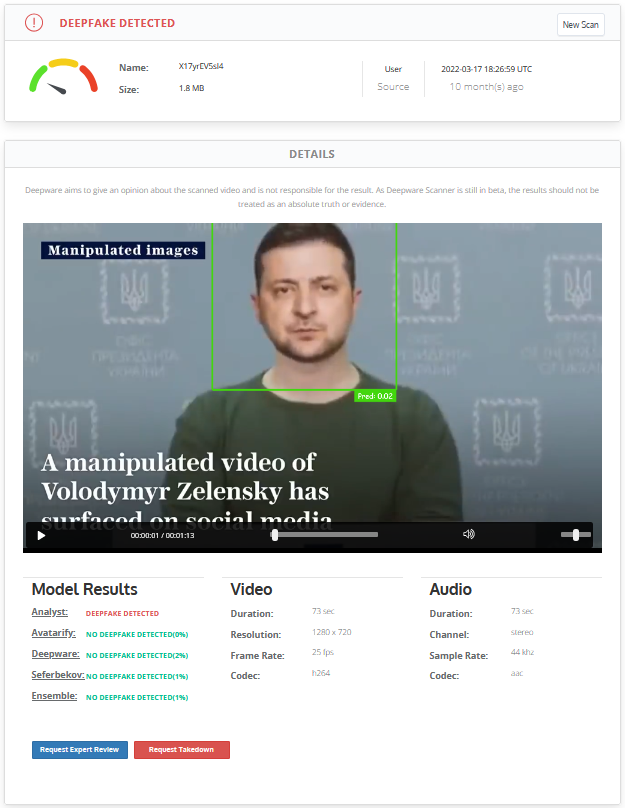
\includegraphics[width=.58\linewidth]{other-fig/deepware_results.png}        
    \caption{Results of Deepware scanner containing probability of deepfakes from multiple detection methods}
    \label{fig:deepware_results}
\end{figure}

The Web application is stating that the project is in Beta, but unfortunately the last commit to the GitHub repository was mad on 7th of June reported at the time of writing this thesis.

The tool provides a simple user interface to scan only videos. The user can input the link to the video (e.g. YouTube) or upload the video file directly as shown in Fig. \ref{fig:deepware_input} . There are many supported video formats. The only limitation is the length of the video, which does not have to be longer than 10 minutes.

Processing of approximately 1 minute long video takes several seconds (3-10 seconds). Results contains video and audio metadata, results of multiple detection methods/models, and deciding whether it is a deepfake or not with gauge chart of confidence as we can observe in Fig \ref{fig:deepware_results}. To use their Rest API, you need to request authentication token. API provides the same functionality as web UI via three methods.

\begin{itemize}
\item POST /video/scan
\item GET /url/scan
\item GET /video/report
\end{itemize}

The first two methods execute scan on a video file or link and return report ID. Results report could be retrieved by last method and results are returned as JSON. Documentation also code samples for multiple programming languages on how to use API properly. The provided API can be integrated to other processes like mail communication scans or file upload filters.

\subsection{Sensity}

Sensity is very similar from the user perspective to Deepware. Based on the post on Sensity blog \cite{HowToDetectADeepfakeOnline} from 2021 we can explore web UI of their application. The application is not publicly accessible and to obtain access, you need to request it. Sensity provides more tools related to cybersecurity, person identification, and verification. 

Sensity allows for detection of images and videos by inserting files or referencing them via a URL link as shown in Fig. \ref{fig:sensity_input}. Sensity allows processing of quite small group of file types (png, jpeg, jfif, tiff, mp4, mov). Another limitations are for videos regarding their size (up to 30MB), length (10 minutes), and quality of videos (1440p). \cite{HowToDetectADeepfakeOnline}

\begin{figure}[H]
    \centering
    
\includegraphics[width=.85\linewidth]{other-fig/sensity_input.png}        
    \caption{Sensity deepfake detection tool input form. Retrieved from \cite{HowToDetectADeepfakeOnline}.}
    \label{fig:sensity_input}
\end{figure}

The tool is capable of recognize only face swap and fully synthesized faces by GAN. It is not able to recognize morphed images or other deepfakes. For GAN-genereated faces, it is sometimes able to classify model generator. If deepfake is recognize tool show how confident he is, all shwon in Fig. \ref{fig:sensity_results}. Compared to Deepware, it provides image scans; on the other hand, it does not have mobile application.

\begin{figure}[H]
    \centering
    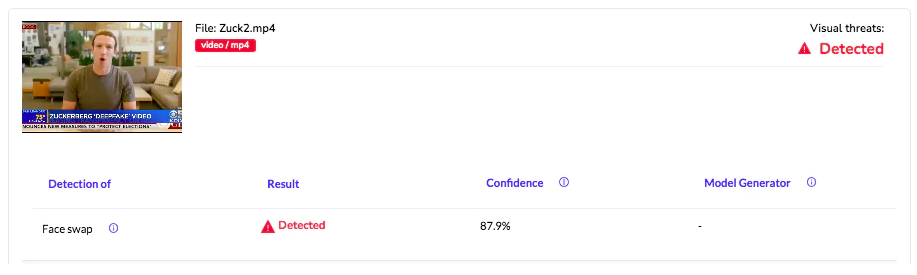
\includegraphics[width=.9\linewidth]{other-fig/sensity_results.png}        
    \caption{Sensity deepfake detection tool results. Retrieved from \cite{HowToDetectADeepfakeOnline}.}
    \label{fig:sensity_results}
\end{figure}

\chapter{Architecture and technologies analysis}

The goal of this work is to develop a deepfake detection framework capable of serving various client applications and an exemplary web plugin subscribing this framework. We already analyze the market and test existing tools. Because there is no external contracting party defining their need, we will define requirements by ourselves. Requirements will be divided into two categories, functional and non-functional requirements. It is important to define not only functional logic, but also some limits on processing time, number of users, etc.

\section{Requirements}

As we already said, the framework has to support multiple clients, so there needs to be a properly defined communication interface between the client applications and the framework itself, which will act as server in this case. Framework allows dynamic changing detection methods, which means it is able to add, remove, or edit detection method. This implicates multiple detection methods at one time for image, video, and even voice deepfake detection. Editing detection method means updating the model or constant parameters. 

The platform should support as many file types as possible and adding a new method should not affect methods already presented in the framework, within supported file types. Different detection methods have different models depending on their design, so model management will be wrapped completely into the detection method.

The framework should collect statistics and hardware metrics, but the collection of personal information should be omitted. All collected metrics will be used for future improvements of detection methods and optimizing operating costs and performance. We would like to have a short response time with as low operating costs as possible. Those two parameters are in contradiction, so there has to be some balance between them. Scalability of the framework or some computationally intensive parts of the framework will help with these requirements. From a perspective number of users, the platform will handle up to hundreds of users at one time, and with enough resources the framework should handle even more.

The client application has to be simple so that anyone can use it. Users should be able to upload files or put a link to a file. The Web plugin allows access to DOM of the webpage so an optional extension will be selection of web elements and retrieval from metadata of it automatically. Because it should cover a large group of possible users, results have to be easy to understand and also provides information for experienced users. Last but not least, the client application should enable users to send feedback. There are several web browsers in market that cover almost all audience, it will be nice that the developed web plugin will be portable among multiple web browsers.

Today it is standard, but it is necessary to mention that the application should be secured. It will affect code of framework, client application, and environment itself (hardware, operating systems, …). All work is open-source and accessible on the public GitHub repository.
\\\\
\noindent Summary of functional requirements:
\begin{itemize}
\item Adding, removing, and editing (changing parameters and models) detection methods
\item Multiple detection methods at once
\item Collecting statistics and feedback
\item Detection of image, video, and voice
\item Detection of file, URL link, or selected HTML element (optional)
\item Understandable presentation of results
\item Security    
\end{itemize}

\noindent Summary of non-functional requirements:
\begin{itemize}  
\item Scalability
\item Small response time
\item Low operating costs
\item Portability of the web plugin among multiple web browsers (optional)
\item Open source    
\end{itemize}

\section{Containerazation}

The framework requires dynamic management of the detection methods. It means that the framework can contain one or twenty different detection methods. Each method could be developed using different programming languages or technologies. Also, model management will be integrated into the detection method. This leads to some isolation of each detection method with a defined communication protocol. Another requirement requires scalability of framework, and all this together will be reached via containerization.

There are many technologies dealing with containers, such as Docker, Podman, LXC. When we start counting orchestration with automatic scalability, the number of technologies drops down. Cloud solutions such as AWS, Azure offer Kubernetes for orchestration of Docker containers. In addition, Docker is probably the most widely used technology for containerization. Because of the huge community and good support of different cloud platforms, we can possibly run framework, we will stick with duo Kubernetes and Docker.

\section{Framework}

The framework is a collection of detection methods, an interface for the client application (receiving requests, sending report response), and orchestrates/arranges all communication. It will be built into several containers and one of the containers will be providing client application interface. It could be Rest API, GraphQL or custom protocol. It is not a good idea to develop a custom communication protocol, so we will stick to the most used Rest API. For this purpose, we can use a huge number of different technologies such as ASP.NET Core, Flusk, Django, Ruby on Rails, etc.

Basically all named technologies meet defined requirements (response time, number of users, ect.) because most of them are covered by microservice design and containerization described in chapter X. Our choice is ASP.NET Core because it has a huge community, Linux support, many external libraries, it is suitable for bigger projects, and it has good speed of program development.

\section{Web browser plugin}

Web plugins are based on web technologies such as HTML, CSS, JavaScript, TypeScript, etc. There are also technologies like WebAssembly which allow development of web applications in languages like C++ without usage of web framework. Because of portability and good integration we will choose HTML, CSS, and Typescript. Typescript is a strict syntactical superset of JavaScript and adds optional static typing to the language. It is also compiled into JavaScript. With those technologies we could be able to create portable web plugin for Chromium base browsers and Firefox.

% \section{Selected detection methods}

\chapter{Framework architecture}

\section{Containerazation and scaling}

\section{High level architecture}
\url{https://microservices.io/patterns/microservices.html}
\begin{figure}[H]
    \centering
    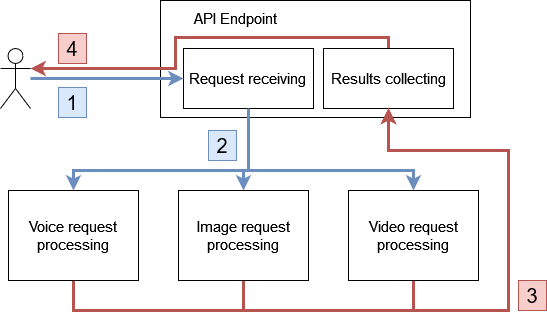
\includegraphics[width=.7\linewidth]{other-fig/framework_architecture.png}        
    \caption{...}
    \label{fig:xxx}
\end{figure}

\begin{figure}[H]
    \centering
    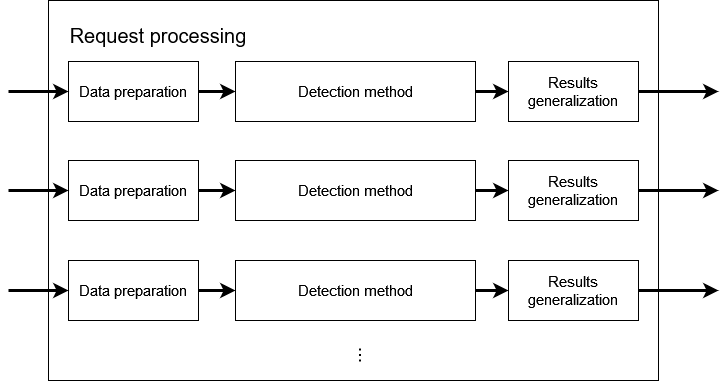
\includegraphics[width=.65\linewidth]{other-fig/framework_architecture_request_processing.png}        
    \caption{...}
\label{fig:xxx}
\end{figure}

\begin{itemize}
\item /ping
    \begin{itemize}
        \item GET /ping – healtcheck
    \end{itemize}
\item /detect
    \begin{itemize}
        \item POST /detect/file – ...
        \item POST /detect/link – ...
    \end{itemize}
\item /progress
    \begin{itemize}
        \item GET /progress/<request\_id> – websocket    
    \end{itemize}
\end{itemize}


% \section{Input layer}

% GET /auth/key
% Authorization token (key) renewal.
% Request Headers
% X-Api-Key: The last auth key token.
% Request Content
% (none)
% Response Code
% 200 OK: the success
% 401 Unauthorized: invalid X-API-Key
% Response Headers
% X-Api-Key: The new auth key token.
% Date: The date and time at which the message was originated (in "HTTP-date" format as defined by RFC 7231 Date/Time Formats).
% Expires: Gives the date/time after which the response is considered stale (in "HTTP-date" format as defined by RFC 7231).
% Response Content
% (none)

% \section{Request processing}
% \subsection{Data preparation layer}
% \subsection{Inividual detection method}
% \subsection{Results generalization}
% \section{Output layer}

\chapter{Client architecture}
\section{Web browser plugin}

\begin{figure}[H]
    \begin{subfigure}[h]{.5\linewidth}
        \centering
        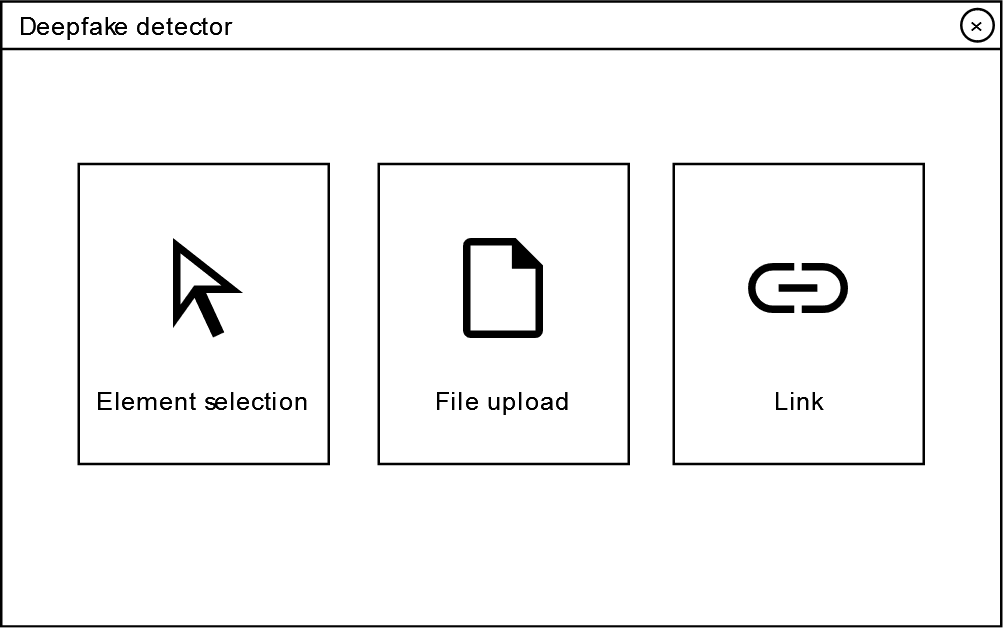
\includegraphics[width=1\linewidth]{other-fig/client_wireframe_input_selection.png}
        \caption{...}
    \end{subfigure}
    \hfill
    \begin{subfigure}[h]{.475\linewidth}
        \centering
        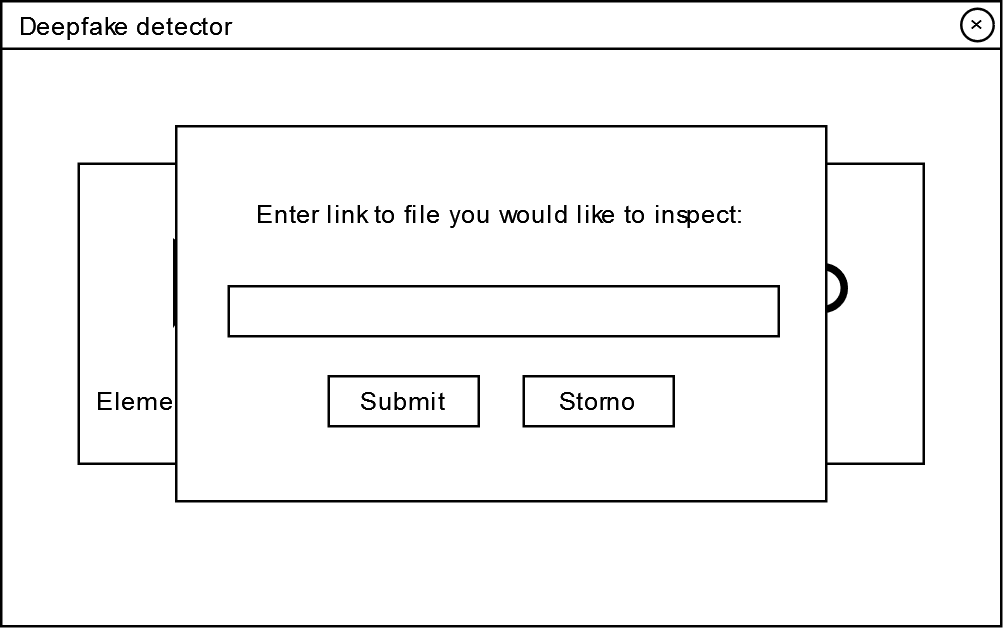
\includegraphics[width=1\linewidth]{other-fig/client_wireframe_input_selection2.png}
        \caption{...}
    \end{subfigure}
    \caption{...}
    \label{fig:xxx}
\end{figure}

\begin{figure}[H]
    \begin{subfigure}[h]{.475\linewidth}
        \centering
        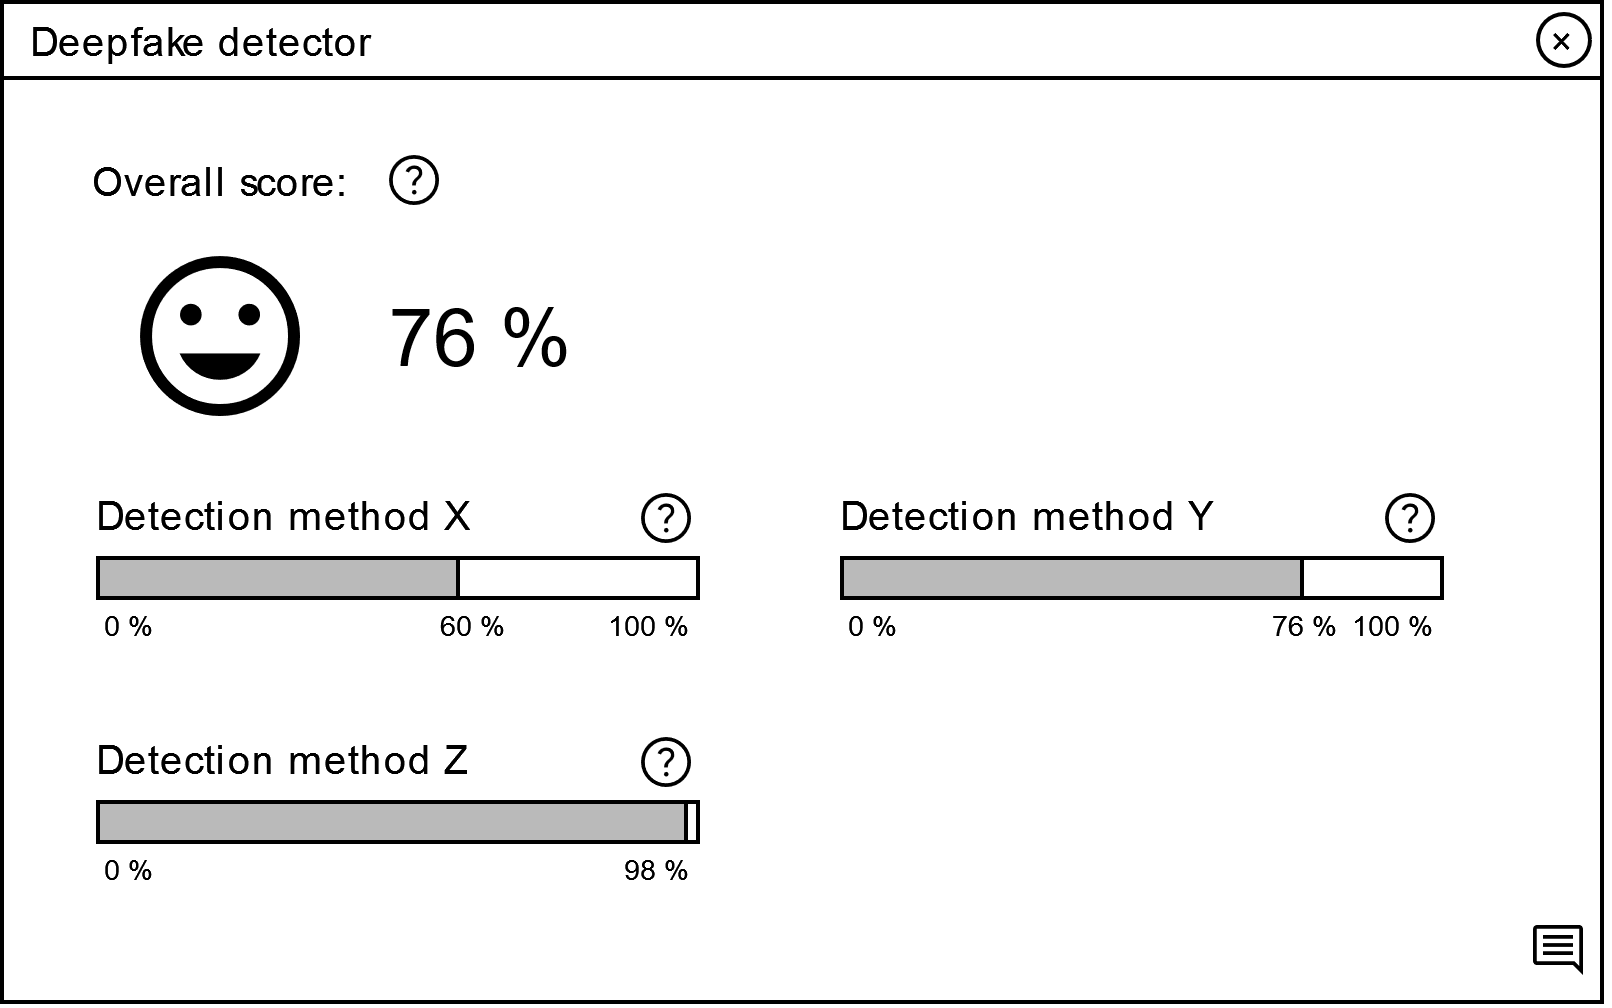
\includegraphics[width=1\linewidth]{other-fig/client_wireframe_results.png}
        \caption{...}
    \end{subfigure}
    \hfill
    \begin{subfigure}[h]{.475\linewidth}
        \centering
        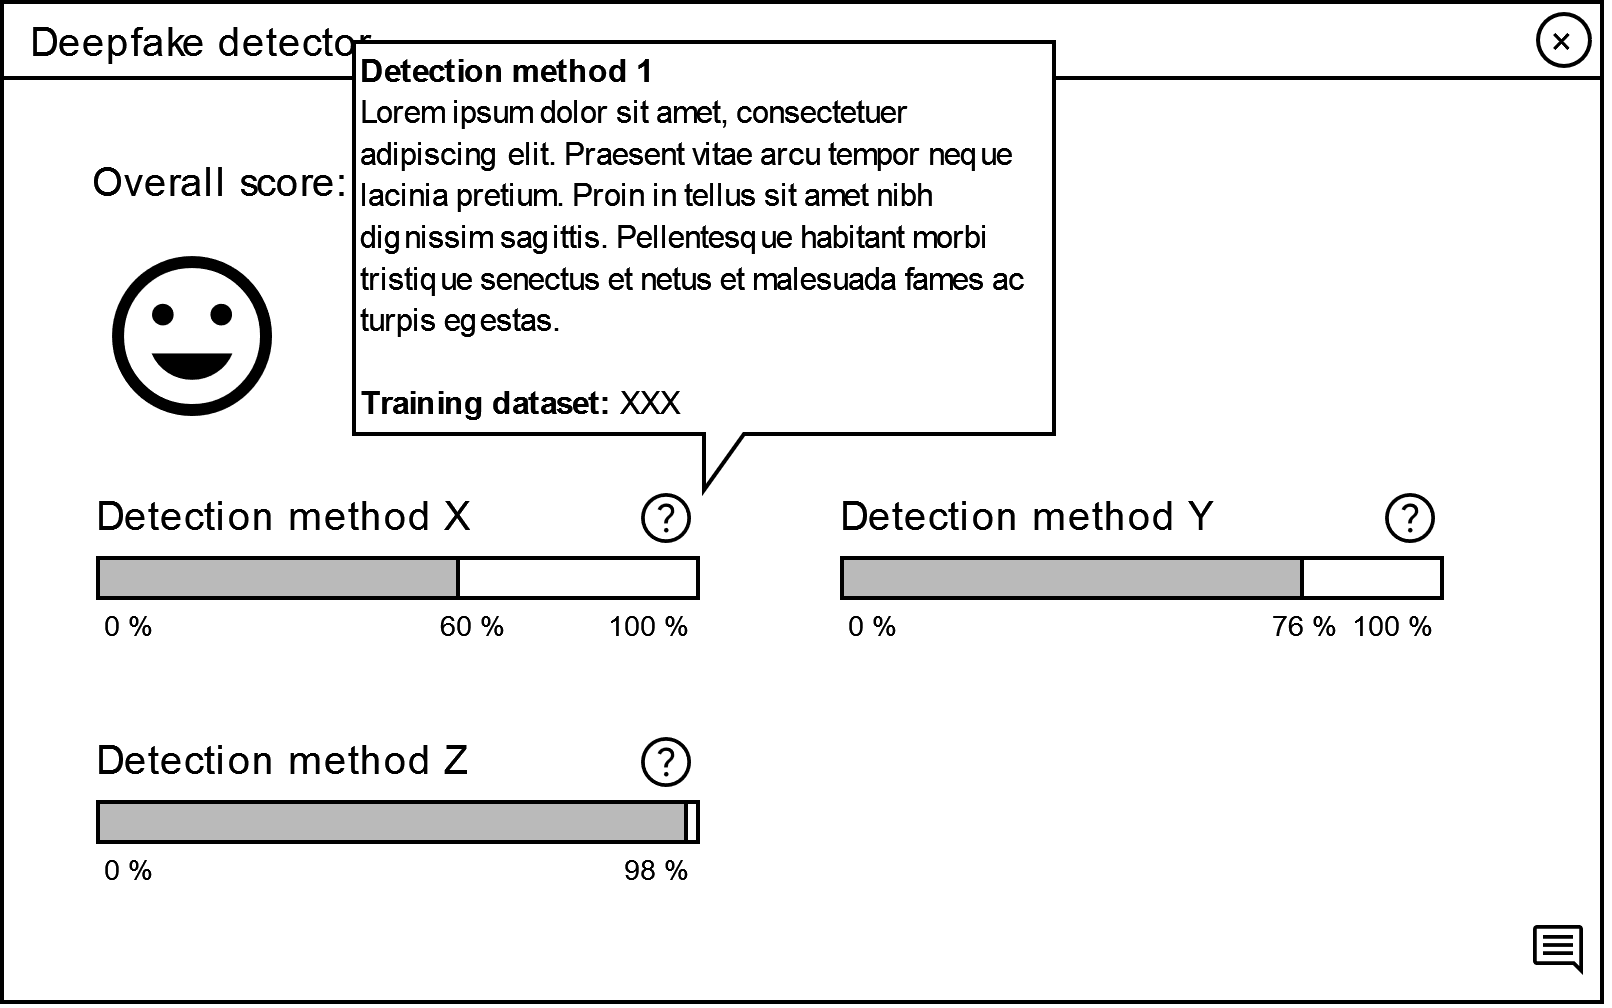
\includegraphics[width=1\linewidth]{other-fig/client_wireframe_results2.png}
        \caption{...}
    \end{subfigure}
    \caption{...}
    \label{fig:xxx}
\end{figure}

\begin{figure}[H]
    \centering
    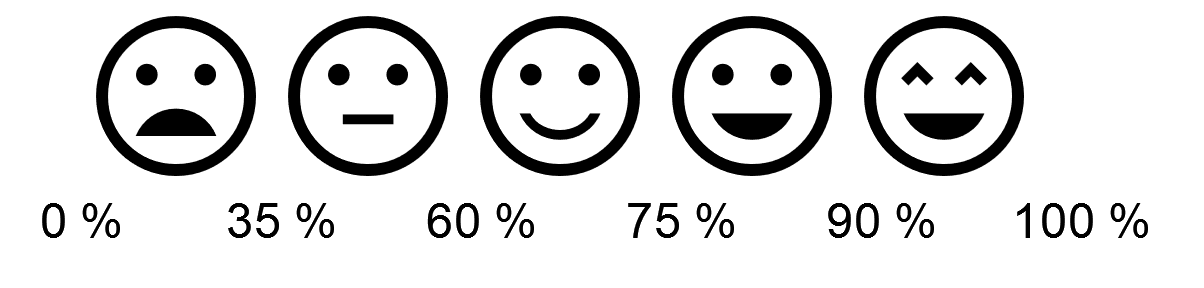
\includegraphics[width=.4\linewidth]{other-fig/client_wireframe_results3.png}        
    \caption{...}
\label{fig:xxx}
\end{figure}

% \chapter{Framework implementation}

% \chapter{Client implementation}

% \chapter{Test experiment and results}

\chapter{Conclusion}